%% ===== Begin LaTeX file ===========================
%%
\documentclass[10pt,a5paper,twoside]{article}
\usepackage{pandoc/coling2012}
\usepackage{color}
\sloppy
\hyphenpenalty 10000
\title{Interface Tangible comme Aide à la Maîtrise de l'Énergie}

\author{Maxime DANIEL\\ Guillaume RIVIÈRE\\ Nadine COUTURE}
\date{\today}


\begin{document}

\maketitle
\keywords{IHM, TUI, technologie persuasive, espace publique physique, gestion de l'énergie}

\clearpage
\tableofcontents
\clearpage
\section{Contexte}\label{contexte}

\subsection{Le développement durable}\label{le-duxe9veloppement-durable}

Le développement durable est le développement qui subvient aux besoins
du présent sans compromettre la capacité des générations futures à
répondre à leurs propres besoins \citep{Hariem1985world}. Face à la
crise écologique et sociale à la quelle le monde fait face (changement
climatique, raréfaction des ressources naturelles, pénuries d'eau douce,
rapprochement du pic pétrolier, écarts entre pays développés et pays en
développement, sécurité alimentaire, déforestation et perte drastique de
biodiversité, croissance de la population mondiale, catastrophes
naturelles et industrielles) atteindre le développement durable est une
priorité indiscutable. Une grande majorité, si ce n'est pas la totalité,
des secteurs d'activités sont concernés par le développement durable.

\subsection{L'énergie}\label{luxe9nergie}

Le secteur de l'énergie est un acteur majeur du développement durable
depuis les premières crises énergétiques des années 1970. En 1973, 86.7
\% de la production mondiale d'énergie primaire provenait des
combustibles fossiles \citep{iea2015key}. À cette époque le système de
production énergétique était presque exclusivement basé sur l'énergie
fossile. Afin d'obtenir ce type d'énergie, il est nécessaire d'exploiter
des combustibles fossiles telles que le pétrole, le charbon ou le gaz
naturel qui sont disponibles en quantité limitée. En 1973, avec une part
de 46.2 \% \citep{iea2015key}, le pétrole était le combustible fossile
le plus utilisée dans le monde et à l'arrivé du premier choc pétrolier
de cette même année, le monde a fait l'expérience d'une pénurie de
pétrole, sa source d'énergie fossile principale. En plus du problème des
réserves limitées des combustibles fossiles, l'exploitation de ces
combustibles produit une grande quantité de polluant et contribue en
grande partie au réchauffement climatique. À la suite de ces évènements,
le secteur de l'énergie à entrepris la recherche d'énergies alternatives
à l'énergie fossile afin de réduire la dépendance aux combustibles
fossiles disponibles en quantité limité et réduire l'impact
environnementale (e.g., pollution, réchauffement climatique) de la
production de cette énergie. L'énergie nucléaire et l'énergie
renouvelable sont deux énergies alternatives à l'énergie fossile issues
de cette recherche.

L'énergie renouvelable est une énergie produisant pas ou très peu de
polluant et dont les ressources sont considérées comme inépuisables. Il
existe différents types d'énergie renouvelable telles que l'énergie
solaire, l'énergie éolienne, l'énergie hydraulique, la biomasse ou
encore l'énergie géothermique. En 2013, l'énergie primaire mondiale
produite était à 13.8 \% de l'énergie renouvelable, 4.8 \% de l'énergie
nucléaire et à 81.4 \% de l'énergie fossile \citep{iea2015key}.
L'énergie renouvelable fait partie du paysage énergétique mondiale et
forme avec l'énergie fossile et l'énergie nucléaire le mix énergétique.

En 40 ans, la part de l'énergie renouvelable dans le mix énergétique est
passé de 12.4 \% en 1973 à 13.8 \% en 2013 \citep{iea2015key}. Cette
lenteur dans la transition vers les énergies renouvelables, est la
conséquence d'une continuité dans l'exploitation des combustibles
fossiles dont l'économie restent, encore aujourd'hui, considérables mais
pas seulement. Les réseaux électriques classiques sont également
responsables de cette lenteur dans la transition énergétique vers le
renouvelable. Ils se montrent particulièrement inadaptés à l'intégration
des énergies renouvelables au paysage énergétique. Cette inadaptabilité
s'expliquer par la variabilité de certaines énergies renouvelables
(solaire, éolien, etc.) qui pose de réels problèmes de gestion de la
production d'électricité ou encore par la multiplication des sites de
production d'électricité (i.e.~décentralisation de la production
d'électricité) qui n'est pas adapté aux réseaux électriques classiques
qui sont conçus pour acheminer et non pour collecter l'électricité.
\textcolor{red}{à continuer vers smart grid et le besoin d'engager les consommateurs + références}

\subsection{L'interaction
homme-machine}\label{linteraction-homme-machine}

\citet{Blevis2007sustainable} évoque le besoin de changer le rôle joué
par l'IHM dans les cycles rapides d'obsolescence des produits qui
contribuent entre autres à la raréfaction des ressources naturelles et à
la pollution. Il expose la possibilité de réduire l'impact matériel de
la technologie à la fois directement (e.g., par la création de produit
qui peuvent être remplacer partiellement plutôt que complètement) et
indirectement (e.g., par la création de produits à qualité héréditaire
afin qu'ils ne soient pas rapidement remplacés).
\citet{mankoff2007environmental} offre une catégorisation de l'IHM pour
le développement durable en deux catégories : le développement durable
\emph{dans} la conception (mitiger l'impact matériel du
logiciel/matériel) et le développement durable \emph{par} la conception
(influencer les styles de vie et les prises de décision durables).
\citet{Reitberger2008surrounded} et \citet{Tscheligi2007persuasion}
affirment que la technologie persuasive peut être un ingrédient clé de
l'IHM pour le développement durable en informant les utilisateurs sur
l'impact environnemental de leurs actions et en augmentant la
désirabilité des comportements pro-environnementaux.
\textcolor{red}{à continuer plus en détails vers les technologies persuasives + références}

\section{Problématique}\label{probluxe9matique}

\begin{enumerate}
\def\labelenumi{\arabic{enumi}.}
\itemsep1pt\parskip0pt\parsep0pt
\item
  Pour persuader les individus à changer de comportement, beaucoup de
  travaux en technologie persuasive utilisent une stratégie de
  persuasion avec comme source principale de motivation, la réduction de
  la facture énergétique du domicile.
\item
  Les individus ne se sentent pas concernés par la réduction de la
  facture énergétique sur les espaces publiques physiques (une école,
  une entreprise, un hôpital, etc.) ; l'application de la technologie
  persuasive sur ces espaces est quelque peu délaissée.
\item
  D'autres sources de motivation commencent à être utilisées telles que
  le plaisir avec l'utilisation de la ludification, voir même du
  \emph{Serious Game}.
\item
  Les interfaces graphiques (GUI) sont majoritairement utilisées comme
  support aux technologies persuasives. Cependant, il existe d'autres
  types d'interfaces homme-machine telles que les interfaces utilisateur
  tangibles qui pourraient se montrer plus adaptées au support des
  technologies persuasives que les GUIs pour certaines situations (e.g.,
  support aux technologies persuasives sur les espaces publiques
  physiques).
\end{enumerate}

\section{État de l'art}\label{uxe9tat-de-lart}

\subsection{Technologie persuasive}\label{technologie-persuasive}

\begin{enumerate}
\def\labelenumi{\arabic{enumi}.}
\itemsep1pt\parskip0pt\parsep0pt
\item
  Définition de la technologie persuasive par \citet{fogg1998captology},
  \citet{fogg2002persuasive}.
\item
  Définition du \emph{Serious Game} par \citet{abt1970serious},
  \citet{ritterfeld2009serious} et de la ludification par
  \citet{deterding2011game}.
\item
  Définition des systèmes ludo-persuasifs par
  \citet{senach2015systemes}.
\item
  Applications :

  \begin{itemize}
  \itemsep1pt\parskip0pt\parsep0pt
  \item
    Santé - \textcolor{red}{à lire} \citet{bhatnagar2012biometric},
    \citet{chiu2009playful}, \citet{fabri2013changing},
    \citet{gasca2008persuasive}, \citet{halan2010high},
    \citet{kehr2012transformational}, \citet{kroes2013empowering},
    \citet{lee2011mining}, \citet{looije2006incorporating},
    \citet{nakajima2013designing}, \citet{parmar2008persuasive},
    \citet{salam2010using}, \citet{vanleer2012use} -.
  \item
    Exercices -\textcolor{red}{à lire} \citet{arteaga2010mobile},
    \citet{berkovsky2012physical}, \citet{consolvo2008flowers},
    \citet{consolvo2008activity}, \citet{foster2010motivating},
    \citet{lacroix2009understanding}, \citet{lim2010pediluma},
    \citet{mutsuddi2012text}, \citet{ploderer2008hey},
    \citet{young2010twitter} -.
  \item
    Éducation, apprentissage - \textcolor{red}{à lire}
    \citet{berque2011design}, \citet{chang2008playful},
    \citet{goh2012impact}, \citet{lucero2006persuasive},
    \citet{reis2011perception} -.
  \item
    Économie, commerce, marketing - \textcolor{red}{à lire}
    \citet{cugelman2008website}, \citet{russell2008benevolence} -.
  \item
    sécurité, sûreté - \textcolor{red}{à lire}
    \citet{bergmans2013reducing}, \citet{chittaro2012passengers},
    \citet{hartwig2013safety}, \citet{miranda2013examining} -.
  \item
    Divertissement - \textcolor{red}{à lire}
    \citet{centieiro2012applaud}, \citet{reitberger2012persuasive} -.
  \item
    Consommation et/ou comportement écologique - \textcolor{red}{à lire}
    \citet{centieiro2011location}, \citet{ruijten2012bridging} -.
  \item
    Gestion de l'énergie - \citet{ham2010ambient},
    \citet{medland2010curbing} , \citet{rodgers2011exploring},
    \citet{gamberini2012tailoring}, \citet{costanza2012understanding},
    \citet{weiss2009handy}, \citet{pereira2013understanding},
    \citet{elsmore2010neighbourhood}, \citet{petkov2012personalised},
    \citet{kjeldskov2012using}, \citet{paay2014design},
    \textcolor{red}{à lire} \citet{filonik2013customisable},
    \citet{foster2010wattsup}, \citet{gamberini2012tailoring},
    \citet{kim2010design}, \citet{roubroeks2010dominant},
    \citet{ruijten2012bridging}, \citet{ruijten2011unconscious},
    \citet{valkanova2013reveal} -.
  \end{itemize}
\item
  Modèle de persuasion de \citet{kaptein2010persuasion} composé du
  modèle de la probabilité d'élaboration de
  \citet{petty1986elaboration}, de la théorie Motivation, Opportunité,
  Capacité de \citet{maclnnis1989information}, de la théorie du
  comportement planifié de \citet{dillon1996user}, du conditionnement
  classique de \citet{patterson1987rabbit} et du conditionnement opérant
  de \citet{skinner1976behaviorism}.
\item
  Modèle de conduite du changement comportemental de
  \citet{prochaska2005transtheoretical}.
\item
  Principes de persuasion de \citet{negri2015ludo} inspirés par les
  principes de persuasion de \citet{fogg2002persuasive},
  \citet{oinas2009persuasive}, \citet{nemery2012development},
  \citet{cialdini2004influence} et les principes de ludification de
  \citet{zichermann2011gamification}.
\item
  Espace de classification de \citet{cano2015persuasive}.
\end{enumerate}

\subsection{Interface utilisateur
tangible}\label{interface-utilisateur-tangible}

\begin{enumerate}
\def\labelenumi{\arabic{enumi}.}
\item
  Définition des TUIs - \citet{wellner1993back},
  \citet{fitzmaurice1995bricks}, \citet{ishii1997tangible},
  \citet{ullmer2000emerging}, \citet{shaer2010tangible} -.
\item
  Applications et exemples :

  \begin{itemize}
  \itemsep1pt\parskip0pt\parsep0pt
  \item
    Communication sociale - \citet{werner2008unitedpulse},
    \citet{ernevi2005interactive}, \citet{chang2001lumitouch} -.
  \item
    Apprentissage - \citet{zufferey2009tinkerSheets},
    \citet{underkoffler1998illuminatinglight}, \citet{raffle2004topobo},
    \citet{frei2000curlybot} -.
  \item
    Divertissement et éducation - \citet{zigelbaum2007tangible},
    \citet{ryokai2004iobrush}, \citet{frey2014teegi},
    \citet{gervais2015tobe} -.
  \item
    Musique et Performance - \citet{jorda2007reactable},
    \citet{schiettecatte2008audiocubes}, \citet{patten2002audiopad},
    \citet{newton2003block} -.
  \item
    Planification et résolution de problème - \citet{ishii2008tangible},
    \citet{underkoffler1999urp}, \citet{patten2007mechanical},
    \citet{jacob2002tangible} -.
  \item
    Programmation - \citet{suzuki1995interaction},
    \citet{horn2008tangible}, -.
  \item
    Visualisation d'information - \citet{couture2008geotui},
    \citet{hinckley1994passive} -.
  \end{itemize}
\end{enumerate}

\subsection{Technologie persuasive
ambiante}\label{technologie-persuasive-ambiante}

\subsubsection{Origines}\label{origines}

\citet{fogg2002persuasive} affirme que les technologies persuasives
dédiés aux appareils mobiles sont les plus efficaces lorsqu'il s'agit
d'assister les utilisateurs dans leurs démarches volontaires de
changement attitudinale et/ou comportementale. Cependant, quand il
s'agit d'engager les utilisateurs dans une démarche de changement
attitudinale et/ou comportementale, l'utilisation d'appareils mobiles
comme outils de persuasion
\citep{fogg1998persuasive}\citep{fogg2002persuasive} devient moins
efficace. En effet, pour qu'un individu adopte un outils de persuasion
(i.e.~s'engager dans une démarche de changement attitudinale et/ou
comportementale) cela nécessite généralement de la motivation et des
efforts cognitives de sa part (e.g., installer l'application, lancer
l'application, comprendre les informations de l'application, utiliser
les fonctionnalités de cette application). Or dans beaucoup de
situations journalières les individus n'ont pas la motivation ou manque
de capacités cognitives pour traiter consciemment des informations
relativement complexes (e.g., les nombres représentant la consommation
d'énergie en kWh) \citep{wyer1997automaticity}. Les appareils mobiles ne
sont donc pas les outils de persuasion les plus favorables à
l'engagement de l'utilisateur et au maintient de ce dernier dans une
démarche de changement attitudinale et/ou comportementale, .

Une alternative à l'utilisation des appareils mobiles est d'utiliser les
environnements bâtis telles les espaces publiques ou semi-publiques pour
y intégrer des outils de persuasion. De cette manière, les outils de
persuasion intégrés à l'environnement physique sont capables de
transmettre des suggestions simples aux utilisateurs exactement au bon
moment, au bon endroit et sans les ennuyer
\citep{intille2004ubiquitous}. \textcolor{red}\#\{inaccessible !!!\}
\citet{mathew2005using} utilise cette approche qu'il appel
\emph{persuasion environnementale} dans un contexte de promotion de
l'activité physique. Il propose d'animer l'escalier d'une station de
métro par l'utilisation de verres translucides et d'un dispositif
d'affichage d'information intégré à l'escalier. Lorsqu'un individu
marche sur une des marches de l'escalier, cette marche s'illumine pour
récompenser le comportement de l'individu. De cette manière, l'escalier
incite les passants à prendre l'escalier et contribue à réduire
l'utilisation de l'escalateur au profit de l'utilisation de l'escalier.
Intégrer les technologies persuasives dans les espaces publiques permet
la \emph{persuasion incrémentale} : ``La persuasion est initié par des
éléments persuasifs mais le changement de comportement est le résultats
d'une prise de conscience croissante par rapport à l'importance de ce
changement.'' \citep{mathew2005using}. Comme l'explique
\citet{davis2008towards}, une telle approche peut influencer le
comportement d'individus qui initialement n'étaient pas engagés dans une
démarche de changement attitudinale et/ou comportementale, et ouvre des
possibilités pour l'attractivité, l'amusement, l'ambiguité, et la
subtilité qui sont des qualités qui peuvent rendre un outil de
persuasion intriguant plutôt qu'ennuyant.

\citet{ishii1997tangible} définit l'affichage ambiant comme la
représentation d'information dans l'espace par des changements subtiles
de lumière, de son, ou encore par des mouvements.
\citet{wisneski1998ambient} affirme que l'affichage ambiant permet de
sensibiliser les utilisateurs à travers l'environnement physique, sans
demander l'attention de ces derniers. Comme l'expose
\citet{davis2008towards}, l'affichage ambiant semble être
particulièrement adapté pour intégrer les outils de persuasion dans
l'environnement physique et semble compatible avec l'idée de
désennuiement et de persuasion incrémentale. \citet{davis2008towards}
nomme ce sous domaine des technologies persuasives mêlant affichage
ambiante et technologie persuasive, la \emph{technologie persuasive
ambiante}.

À la suite, certains travaux ont investi l'efficacité des feedbacks
demandant des efforts cognitifs faibles telles que les changements
lumineux utilisés par les affichages ambiants. Concrètement,
\citet{ham2009can} présentent des évidences sur la capacité de la
technologie persuasive à persuader les utilisateurs sans recevoir
consciemment l'attention de ces derniers. Dans une série d'essais, des
participants devaient indiquer quel appareil parmi trois appareils
électro-ménager consommait la plus faible quantité d'énergie moyenne.
Après chaque choix, les participants de la condition feedbacks
supraliminales recevaient un feedback sur la précision de leur réponse
par la présentation d'un visage souriant ou triste pendant 150 ms. Les
participants de la condition feedbacks subliminales recevaient les même
feedback mais seulement pendant 25 ms ce qui empêche la perception
consciente de ces stimuli. Finalement, les participants de la condition
sans feedback ne recevaient aucun feedback. L'expérience montre que
recevoir des feedbacks subliminaux et supraliminaux mène à une meilleur
évaluation de la consommation énergétique moyenne des appareils
électro-ménagers que de ne pas recevoir de feebacks. Cela suggère que la
technologie persuasive ambiante peut être efficace \emph{sans recevoir
consciemment l'attention des utilisateurs}.

Par la suite, \citet{ham2010ambient} approfondit la définition de la
technologie persuasive ambiante et affirme que la technologie persuasive
ambiante peut être également efficace \emph{avec une faible quantité de
ressources cognitives}. Il affirme que les feedbacks lumineux sont plus
simples à traiter que les feedbacks factuels (e.g., les nombres
représentant la consommation en kWh) qui nécessitent plus de ressources
cognitives pour être traiter et évaluer par les utilisateurs. Il
démontre cette hypothèse par une expérience où la moitié des
participants devaient programmer un thermostat qui présentait une
lumière colorée pour indiquer le niveau absolu de consommation
énergétique allant du vert (i.e.~consommation énergétique faible) au
rouge (i.e.~consommation énergétique élevée). L'autre moitié des
participants, quand à eux, devaient programmer un thermostat qui
présentait un premier nombre pour indiquer le niveau absolu de
consommation énergétique en Watts et deux autres nombres représentants
respectivement le niveau de consommation énergétique faible en Watts et
le niveau de consommation énergétique élevée en Watts. Les résultats de
cette expérience montrent que les participants qui ont reçus des
feedbacks lumineux ont utilisés moins d'énergie dans la tâche de
programmation du thermostat que les participants qui ont reçus des
feedbacks factuels. Les résultats suggèrent également que les
participants qui ont reçus les feedbacks factuels ont traités plus
lentement ces feedbacks que les participants qui ont reçus les feedbacks
lumineux comme l'hypothèse le suggérait. En conclusion,
\citet{ham2010ambient} définit les technologies persuasives ambiantes
comme des technologies persuasives intégrés discrètement dans
l'environnement qui exercent une influence sur les individus sans
nécessité leur attention focale (l'attention focale est un type
d'attention dans lequel l'individu est délibérément et consciemment
concentré sur un stimulus tout en excluant les images et sons
environnants).

\subsubsection{\emph{Virtual Aquarium} de
\citet{nakajima2008reflecting}}\label{virtual-aquarium-de-nakajima2008reflecting}

\paragraph{Description}\label{description}

\emph{Virtual Aquarium} cherche à améliorer l'hygiène dentaire des
utilisations par la promotion de pratiques correctes de brossage des
dents. Le système est intégré dans la salle de bain et transforme un
mirror en un aquarium virtuel. Les poissons vivent dans l'aquarium et
sont affectés par l'activité de brossage des dents des utilisateurs. Si
les utilisateurs brossent leurs dents correctement, les poissons
prospèrent et procréent. Sinon les poissons s'affaiblissent et peuvent
même mourir.

\paragraph{Conception}\label{conception}

\begin{figure*}
\centering
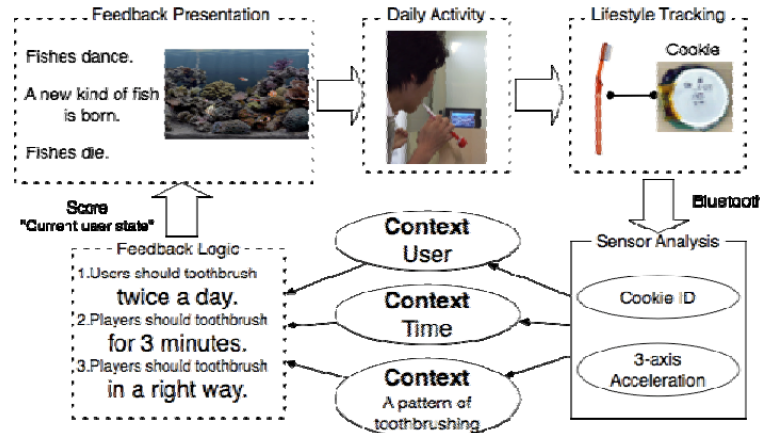
\includegraphics[width=0.900\hsize]{images/virtualaquarium-screenshot2.png}
\caption{Architecture du \emph{Virtual
Aquarium}}\label{fig:virtualaquarium1}
\end{figure*}

Architecture du système (voir Figure~\ref{fig:virtualaquarium1}) :

\begin{itemize}
\itemsep1pt\parskip0pt\parsep0pt
\item
  \textbf{Suivi du style de vie :} L'activité de brossage des dents est
  détectée par des \emph{Cookies} (appareils de la taille d'une pièce
  qui contiennent des capteurs et une interface Bluetooth
  \citep{kimura2006cookieflavors}). Dans ce système, un accéléromètre à
  3 axes est intégré à un Cookie. Un Cookie est attaché à chaque
  brosse-à-dents du foyer. Étant donné que chaque brosse-à-dents n'est
  pas partagée, chaque Cookie possède un identifiant unique. La
  connection Bluetooth, l'acquisition du contexte et les notifications
  d'événements sont gérés par une framework appelé Prottoy
  \citep{kawsar2005prottoy}. Les patterns de brossage des dents sont
  reconnus par l'analyse des données d'accélération.
\item
  \textbf{logique des Feedbacks :} L'objectif de \emph{Virtual Aquarium}
  est d'améliorer l'hygiène dentaire des utilisations par la promotion
  de pratiques correctes de brossage des dents. Le comportement idéale
  est définit comme : 1) les utilisateurs se brossent les dents au moins
  deux fois par jour; 2) une session de brossage des dents implique au
  moins 3 minutes de brossage ; et 3) brossage doit impliquer des
  patterns qui assurent que les dents sont proprement nettoyées. Le
  système offre un renforcement positif pour encourager le brossage de
  dents et désencourage les utilisateurs à passer le brossage de dents
  par des punition positive et des punitions négatives.
\item
  \textbf{Présentation des feedbacks :} Étant donné le prix d'un
  \emph{AwareMirror} (miroir qui peut également se dédoubler en écran),
  le prototype utilise un petit ordinateur avec un écran plat monté sur
  le miroir de la salle de bain. Le prototype offre deux types de
  feedbacks : le feedback immédiat et le feedback accumulé. Le feedback
  immédiat, lorsque l'utilisateur commence à se brosser les dents, une
  éponge à l'intérieur de l'aquarium commence à nettoyer les algues des
  parois de l'aquarium. Au même moment, un groupe de poisson associé à
  l'utilisateur commence à se déplacer de manière joviale. Quand
  l'utilisateur s'est brossé les dents pendant une période suffisante,
  l'éponge finit de nettoyer et la danse des poissons change pour une
  danse plus élégante. Quand l'utilisateur finit son brossage, les
  poissons finissent leur danse et poursuivent leurs activités normales.
  L'activité des poissons et le mouvement de l'éponge sont conçus de
  façon à fournir des indices à l'utilisateur sur la bonne méthode de
  brossage les dents (voir Figure~\ref{fig:virtualaquarium2}). Le
  feedback accumulé, la santé des poissons est visiblement affectée en
  fonction de la propreté de l'aquarium. Si l'utilisateur néglige le
  brossage de leurs dents, quelques poissons tombent malades et peuvent
  même mourir. À l'inverse, un brossage correcte peut aboutir au dépôt
  d'un œuf par un poisson. Au début, les oeufs ne sont pas enclins à
  éclore. Si l'utilisateur continue à se brosser les dents correctement
  pendant un certain nombre de jours d'affilé, la vitesse d'incubation
  de l'œuf augmente. De cette facon, le feedback accumulé offre des
  indices sur le comportement à adopter et tente de maintenir la
  motivation sur une longue période (voir
  Figure~\ref{fig:virtualaquarium3}).
\end{itemize}

\begin{figure*}
\centering
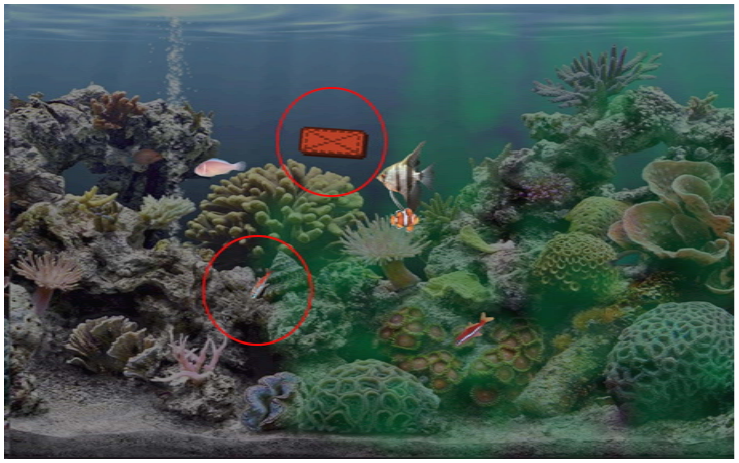
\includegraphics[width=0.900\hsize]{images/virtualaquarium-screenshot3.png}
\caption{\emph{Virtual Aquarium} lorsque l'utilisateur se brosse les
dents.}\label{fig:virtualaquarium2}
\end{figure*}

\begin{figure*}
\centering
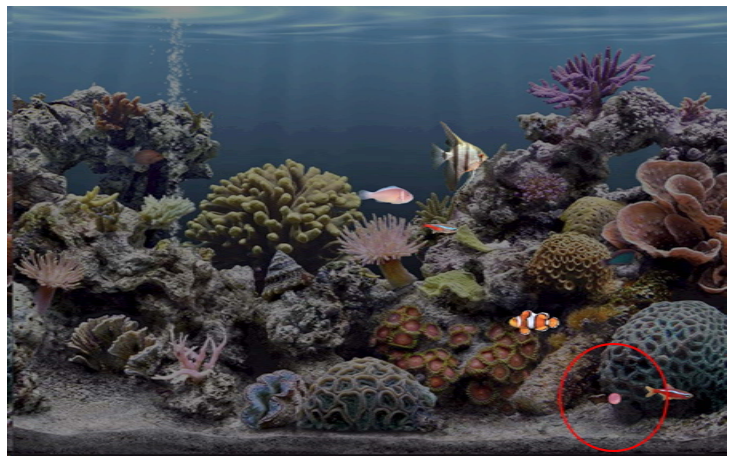
\includegraphics[width=0.900\hsize]{images/virtualaquarium-screenshot4.png}
\caption{Un poisson dépose un œuf au fond du \emph{Virtual
Aquarium}.}\label{fig:virtualaquarium3}
\end{figure*}

\paragraph{Étude}\label{uxe9tude}

Afin d'évaluer les effets de \emph{Virtual Aquarium} une étude pilote a
été effectuée sur 8 à 12 jours, composé de 7 personnes (4 hommes, 3
femmes) provenant de 3 foyers différents. L'étude est divisée en 3
phases :

\begin{itemize}
\itemsep1pt\parskip0pt\parsep0pt
\item
  Dans un ensemble de foyers représentatifs de la population générale,
  un Cookie fut attaché à chaque brosse-à-dents personnelle du foyer.
  Les foyers sont demandés de continuer les activités normales, pendant
  que les patterns de brossage de dents sont enregistrés
  quotidiennement. Une fois les patterns stabilisés au cours du temps,
  l'étude passe à la phase suivante.
\item
  Le \emph{Virtual Aquarium} est introduit dans la salle de bain des
  foyers et les patterns de brossage de dents continuent d'être
  enregistrés quotidiennement. Une fois les patterns stabilisés à
  certain degrés prédéterminé, l'étude passe à la phase finale.
\item
  Le \emph{Virtual Aquarium} est enlevé alors que les patterns de
  brossage de dents continuent d'être enregistrés quotidiennement. Une
  fois les patterns stabilisés à certain degrés prédéterminé les données
  sont collectées. Les données sont alors analysées afin de déterminer
  si l'introduction de \emph{Virtual Aquarium} a eu des effets sur les
  patterns de brossage de dents et à quel point ces effets ont persistés
  dans le temps.
\end{itemize}

\paragraph{Recueil des données}\label{recueil-des-donnuxe9es}

Les données provenant des brosses-à-dents améliorés ont été collectés
pour être analysés.

\paragraph{Résultats (voir
Figure~\ref{fig:virtualaquarium5})}\label{ruxe9sultats-voir-figure}

\begin{figure*}
\centering
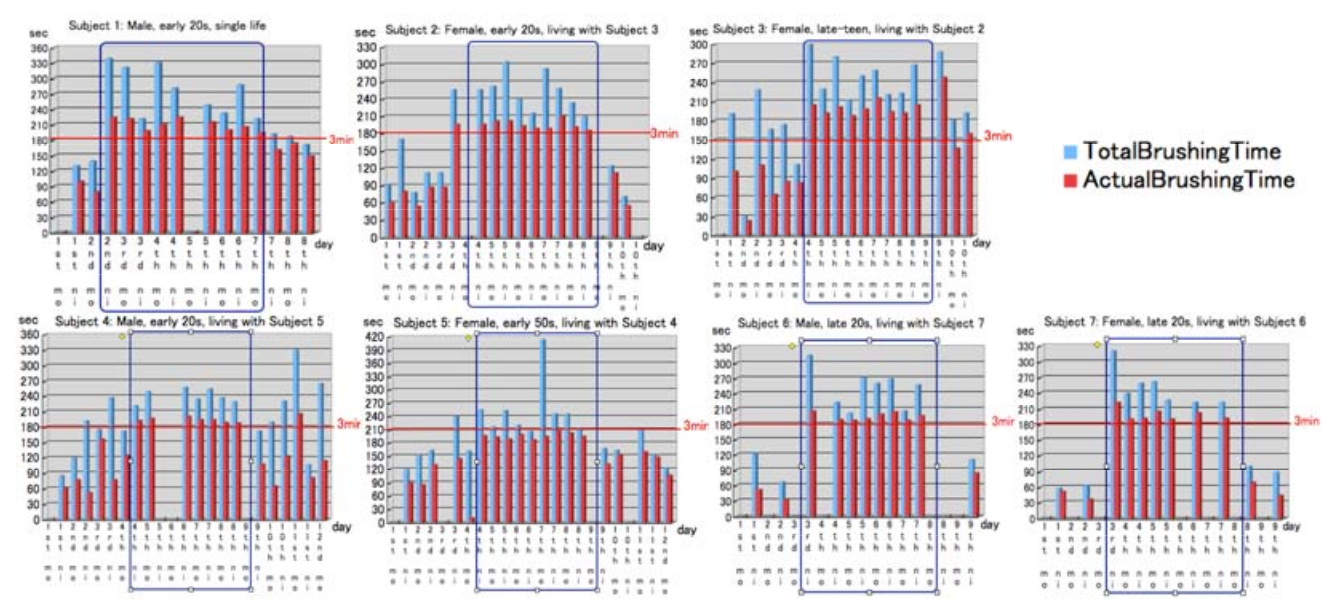
\includegraphics[width=0.900\hsize]{images/virtualaquarium-screenshot5.png}
\caption{Résultats de l'expérience sur le \emph{Virtual
Aquarium}.}\label{fig:virtualaquarium5}
\end{figure*}

\paragraph{Analyse des résultats}\label{analyse-des-ruxe9sultats}

Dans la première phase de l'étude, le temps de brossage était inférieur
à 3 minutes. Dans la deuxième phase, quand \emph{Virtual Aquarium} fut
introduit, le temps de brossage était supérieur à 3 minutes. Dans la
dernière phase, lorsque \emph{Virtual Aquarium} fut enlevé, le temps de
brossage descendit mais tout en restant supérieur au temps de brossage
de la première phase. Les utilisateurs ne pouvaient pas toujours
utiliser le système pour certaines raisons (e.g., se lever trop tard, ne
pas avoir le temps pour se brosser les dents pendant 3 minutes, passer
la nuit autre part qu'au foyer). Les familles étaient intéressées par
l'état de l'aquarium et cela devint un sujet de discussion quotidien
pour ces familles.

\subsubsection{\emph{Mona Lisa Bookshelf} de
\citet{nakajima2008reflecting}}\label{mona-lisa-bookshelf-de-nakajima2008reflecting}

\paragraph{Description}\label{description-1}

Les ressources partagés par des groupes d'individu telles que des
toilettes publiques ou une étagère à livres dans une laboratoire de
recherche, tendent à se détériorer rapidement dans un processus appelé
la tragédie des biens communs. Cela se produit car chaque individu voit
un intérêt personnel à utiliser ces ressources alors que aucuns des
coûts n'est partagés entre les utilisateurs ce qui mène à une
utilisation imprudente de ces ressources. \emph{Mona Lisa Bookshelf}
vise à garder une étagère à livre ordonnée. Il essaye d'encourager les
utilisateurs à garder les livres dans l'ordre et à retourner les livres
manquants mais également à prendre des livres à chaque instant pour les
lire. Chaque livre de l'étagère est lié à une partie d'une image
numérique de \emph{Mon Lisa}. Tel un puzzle, l'image change en fonction
du positionnement des livres. Un écran plat haute qualité placé près de
l'étagère affiche ce puzzle aux utilisateurs.

\subsubsection{Conception}\label{conception-1}

\begin{figure*}
\centering
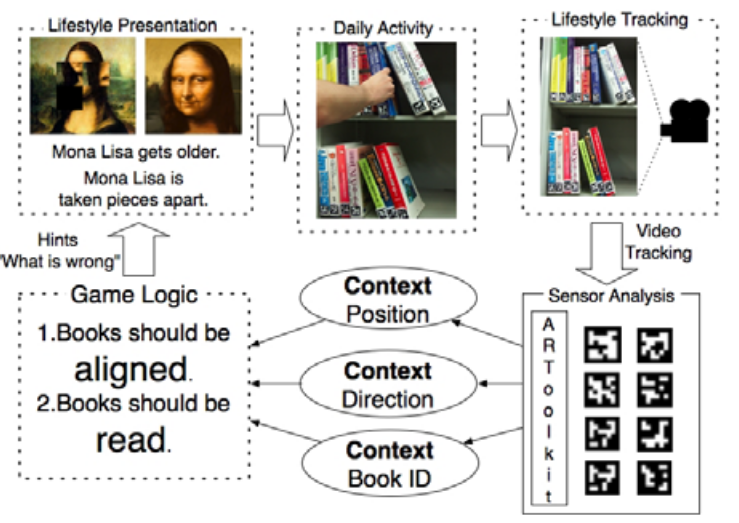
\includegraphics[width=0.900\hsize]{images/monalisa-screenshot1.png}
\caption{Architecture de \emph{Mona Lisa
Bookshelf}}\label{fig:monalisa1}
\end{figure*}

Architecture du système (voir Figure~\ref{fig:monalisa1}) :

\begin{itemize}
\itemsep1pt\parskip0pt\parsep0pt
\item
  \textbf{Suivi du style de vie :} Le traquage est basé sur un détection
  optique des livres de l'étagère. Une étiquette visuelle est attachée à
  chaque reliure des livres pour faciliter la détection et
  l'identification. Des étiquettes visuelles sont également attachées
  sur les bords de l'étagère pour déterminer ses dimensions (voir
  Figure~\ref{fig:monalisa2}). Le système de détection contient : une
  caméra vidéo numérique (iSight de Apple), une caméra numérique haute
  résolution (D50 by Nikon) et deux détecteurs de distance à infrarouge
  (GP2D12 by SHARP). Les capteurs de distances et la caméra vidéo
  numérique sont utilisés pour détecter si un utilisateur manipule des
  livres sur l'étagère. OpenCV est utilisé pour analyser le signal
  vidéo. Aussitôt que l'utilisateur est observé comme quittant la salle,
  la camera numérique haute résolution prend une image de l'étagère et
  des livres qui s'y trouvent. Les images capturées par cette même
  caméra sont analysées par VisualCodes qui permet de reconnaître les
  étiquettes attachées aux livres et leur identité, leur position et
  leur alignement.
\item
  \textbf{logique des Feedbacks :} L'objectif de \emph{Mona Lisa
  Bookshelf} est d'encourager le comportement idéale suivant : 1) les
  livres doivent être rangés correctement et alignés soigneusement
  (e.g., ordre alphabétique); et 2) au moins un des livres doit erre lu
  une fois par semaine. Le système des punitions positives et négatives
  pour encourager l'adoption de comportements souhaités et des
  renforcements négatifs pour décourager l'adoption de comportements non
  souhaités.
\item
  \textbf{Présentation des feedbacks :} Le feeback immédiat, quand un
  livre est enlevé de l'étagère, la partie de l'image de Mona Lisa est
  également enlevée. Si les livres sont allongés sur leur couverture ou
  mal agencés, les parties de l'image deviennent également mal agencées
  et distorde l'image. Quand les livres sont correctement agencés, Mona
  Lisa sourit (voir Figure~\ref{fig:monalisa3}). La supposition est que
  les utilisateurs savent à quoi la \emph{Mona Lisa} de da Vinci est
  supposée ressembler et, tout comme lorsque l'on complète un puzzle,
  les utilisateurs préfèrent l'image complète à l'image distordue. Le
  feedback accumulé, additionnellement à l'effet cumulé des déplacements
  des parties de l'image, il y a un mécanisme de feedback accumulé
  supplémentaire qui tente d'encourager les utilisateurs à lire des
  livres de temps en temps : Si aucun livre n'est enlevé de l'étagère
  pendant plus d'une semaine, Mona Lisa commence à vieillir (voir
  Figure~\ref{fig:monalisa3}). Aussitôt qu'un livre est enlevé de
  l'étagère Mona Lisa regagne sa jeunesse.
\end{itemize}

\begin{figure*}
\centering
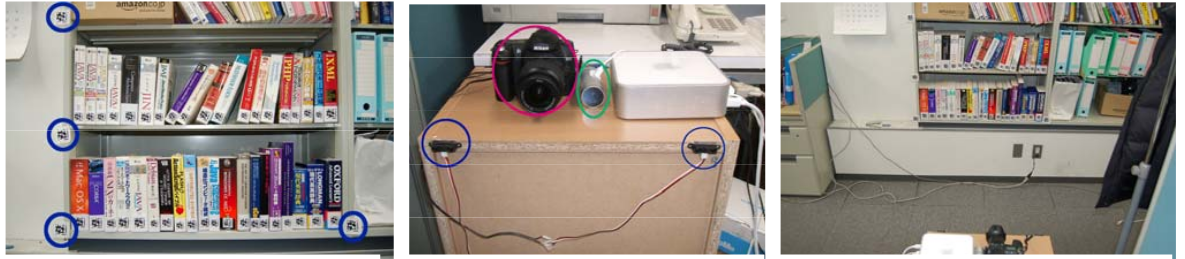
\includegraphics[width=0.900\hsize]{images/monalisa-screenshot2.png}
\caption{Conception de \emph{Mona Lisa Bookshelf}}\label{fig:monalisa2}
\end{figure*}

\begin{figure*}
\centering
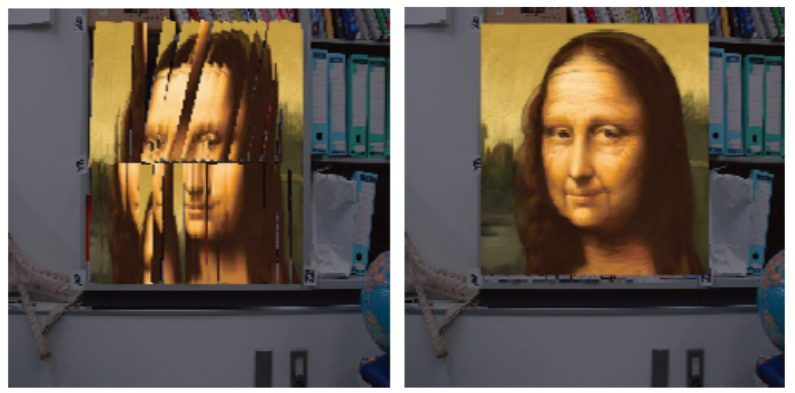
\includegraphics[width=0.900\hsize]{images/monalisa-screenshot3.png}
\caption{\emph{Mona Lisa Bookshelf} in Situ}\label{fig:monalisa3}
\end{figure*}

\paragraph{Étude}\label{uxe9tude-1}

Aucune étude réalisée sur ce prototype.

\subsubsection{\emph{InAir} de
\citet{kim2010inair}}\label{inair-de-kim2010inair}

\paragraph{Description}\label{description-2}

Une faible qualité d'air est difficilement détectable par l'homme que ce
soit par la vue ou l'odeur et peut contribuer au développement de
maladies chroniques. \emph{inAir} est un outil de mesure, de
visualisation et de partage de données sur la qualité d'air en
intérieur.

\paragraph{Conception}\label{conception-2}

\paragraph{Étude}\label{uxe9tude-2}

Afin d'évaluer l'efficacité d'\emph{inAir}, une étude a été effectuée
sur 4 semaines composé de 14 personnes séparées en 6 groupes (2 groupes
de 3 personnes et 4 groupes de 2 personnes). L'étude est divisée en deux
phases : un phase en mode utilisateur et une phase en mode partage. Pour
minimiser l'effet Hawthorne, la moitié des groupes commença par une
phase en mode utilisateur pendant 2 semaines suivie par phase en mode
partage pendant les deux dernières semaines et l'autre moitié des
groupes, quand à elle, a effectuée les phases dans l'ordre inverse.

\paragraph{Recueil des données}\label{recueil-des-donnuxe9es-1}

Pour comprendre les effets cognitifs et comportementaux d'\emph{inAir},
une interview semi-structurelle fut conduite composée de 3 interviews
d'une durée de 30 minutes à 1 heure chacune :

\begin{itemize}
\itemsep1pt\parskip0pt\parsep0pt
\item
  Une interview avant l'étude pour évaluer les connaissances générales
  et la compréhension des participants en matière de qualité de l'air et
  de santé humaine ;
\item
  une interview entre les deux phases pour comprendre comment les
  participants ont intégrés \emph{inAir} dans leur vie et pour
  rassembler des retours sur les changements comportementaux résultants
  de la visualisation des données en temps réel sur la qualité de l'air
  en intérieur ; . et une interview après étude pour repérer des
  différences entre le mode utilisateur et le mode partage, et également
  pour discuter d'éventuelles idées de visualisation de données.
\end{itemize}

\paragraph{Analyse des données}\label{analyse-des-donnuxe9es}

Les résultats des interviews furent analysés selon une approche théorie
ancrée \citep{strauss1990basics}. Leur approche inclus le codage ouvert,
le codage axial et le codage sélectif.

Pendant la phase de codage ouvert, les auteurs ont identifiés des
concepts codés significatifs à partir des données qui correspondent à
des représentations abstraites d'événements, d'objets, d'actions,
d'interactions, etc. Par exemple: ``\emph{Every time factors to worsen
air quality{]} motorcycles {[}/factors to worsen air quality{]} go up or
down on the highway, it spikes. It becomes worse than normal regular
spikes. I can hear them passing by.}'' Un total de 41 concepts furent
crées.

Pendant la phase de codage axial, les auteurs ont catégorisés les
concepts crées pendant la phase de codage ouvert en des phénomènes
conceptuels de plus haut niveau selon un codage axial. Un phénomène dans
la théorie encrée se réfère à des patterns répétés d'évènements,
d'actions, d'interactions qui représente les réponses des participants
faces à des problèmes et des situations. Par exemple, ``augmentation de
la prise de conscience'' est un phénomène qui représentes une
augmentation de la prise de conscience en relation avec les changements
de la qualité de l'air et les causes de ces changements déterminés par
les individus à partir de la visualisation de la qualité de l'air. ``les
facteurs qui diminue la quality de l'air'' est un concept de la phase de
codage ouvert catégorisé en ``augmentation de la prise de conscience''.
Un totale de 7 catégories furent crées.

Pendant la phase de codage sélectif, les auteurs ont assemblés les
phénomènes conceptuelles extraits de la phase de codage axial dans une
unique ligne temporel. L'objectif est de construit des relations entre
les phénomènes.

\begin{figure*}
\centering
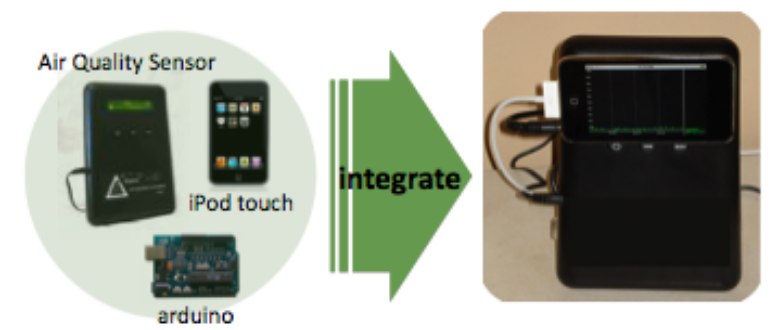
\includegraphics[width=0.900\hsize]{images/inair-screenshot3.png}
\caption{Prototype \emph{inAir}}\label{fig:inair1}
\end{figure*}

\begin{figure*}
\centering
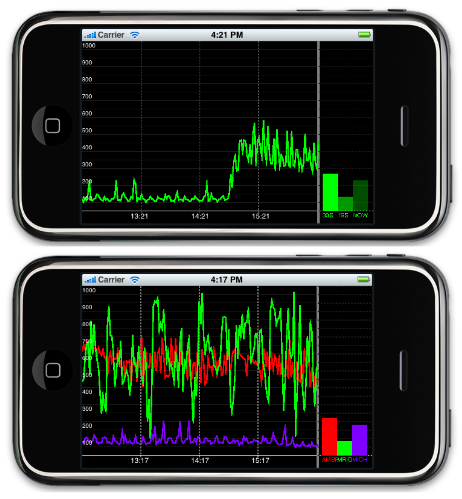
\includegraphics[width=0.700\hsize]{images/inair-screenshot2.png}
\caption{Affichage de \emph{inAir}}\label{fig:inair2}
\end{figure*}

\begin{figure*}
\centering
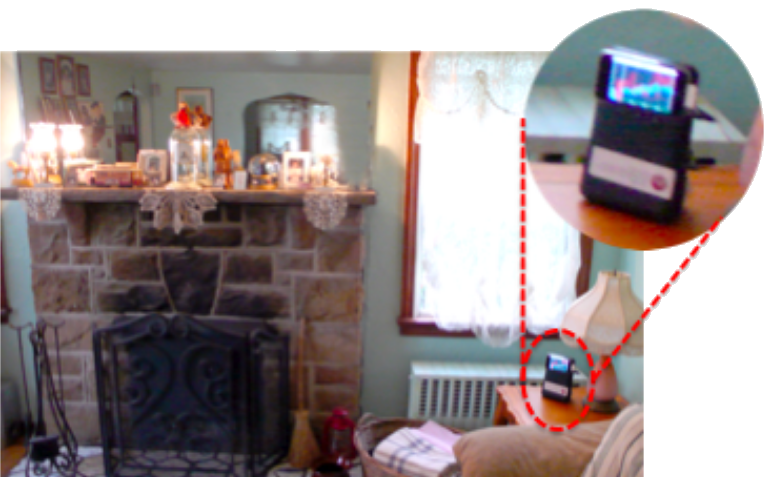
\includegraphics[width=0.900\hsize]{images/inair-screenshot1.png}
\caption{Affichage ambiant de \emph{inAir}}\label{fig:inair3}
\end{figure*}

\begin{figure*}
\centering
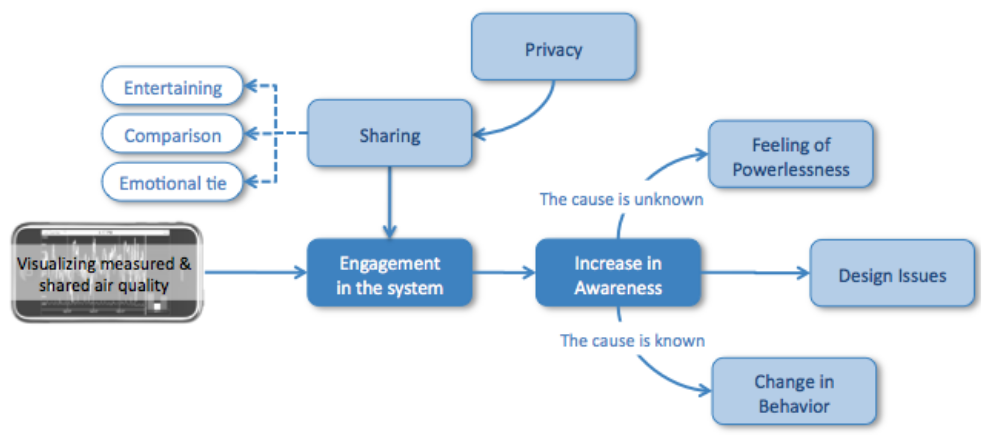
\includegraphics[width=0.900\hsize]{images/inair-diagram.png}
\caption{Modèle diagrammatique des effets d'\emph{inAir} sur les
participants de l'expérience.}\label{fig:inair4}
\end{figure*}

\paragraph{Résultats de l'analyse}\label{ruxe9sultats-de-lanalyse}

Dans leur analyse, les auteurs ont distingués deux catégories majeurs
désignant l'utilité du système, L'``Engagement dans le système'' mène à
l' ``augmentation de la prise de conscience''. D'autres catégories font
référence à la qualité d'\emph{inAir} à engager les individus dans une
démarche de changement comportementale telles que le ``Partage'' qui
motive les individus à atteindre des changements positifs concernant
leur qualité d'air, et renforce les relations sociales. Une catégorie
fait référence au ``Sentiment d'impuissance'' des participants. En
effet, \emph{inAir} crée un sentiment d'impuissance chez les
participants car il est incapable de fournir des informations relatives
à la provenance de la source du problème et ne fournit pas de
suggestions pour améliorer la qualité de l'air.

\subsubsection{\emph{Aulura} de
\citet{faber2011aulura}}\label{aulura-de-faber2011aulura}

\paragraph{Description}\label{description-3}

\emph{Aulura} est un système conçus pour motiver les individus à
accroître leur activité physique. \emph{Aulura} est système d'affichage
ambiant qui vise à séduire les utilisateurs à interagir avec lui pour
visualiser leurs progrès et pour se fixer des défis personnels.

\paragraph{Conception}\label{conception-3}

Les utilisateurs portent un dispositif capable de mesurer leur activité
physique dans le temps. L'activité physique des utilisateurs est
affichée par un indicateur lumineux de progression intégré au cadre du
dispositif où la couleur est utilisé pour identifier l'utilisateur. Des
informations détaillées sont affichées à l'écran. L'identité et le
nombre d'utilisateur présents détermine les informations affichées. La
distance entre les utilisateurs et \emph{Aulura} détermine le mode
d'interaction. L'espace est séparé en différentes zones d'interaction
(voir Figure~\ref{fig:aulura1}) et des informations plus détaillées et
une meilleur interactivité sont offertes aux utilisateurs au fur et à
mesure qu'ils se rapprochent du dispositif.

\begin{figure*}
\centering
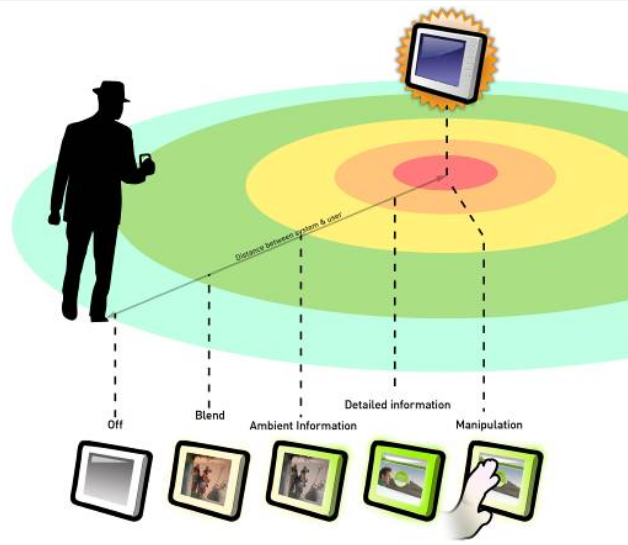
\includegraphics[width=0.900\hsize]{images/Aulura-screenshot.png}
\caption{Zones d'interaction de \emph{Aulura}.}\label{fig:aulura1}
\end{figure*}

Quand l'utilisateur est dans la zone \emph{Blend} le dispositif affiche
une séquence d'images ajoutées personnellement par l'utilisateur. Quand
l'utilisateur est dans la zone \emph{Ambient}, l'activité physique est
visualisé en remplissant graduellement 1 à 4 coins du cadre du
dispositif. Quand l'utilisateur pénètre dans la zone \emph{Details}, la
séquence d'images disparaît pour laisser place à des informations
détaillés sur les accomplissements de la journée tels que le pictogramme
de l'utilisateur, le pourcentage accompli par rapport au niveau
d'activité physique ciblé, les calories brûlées et le temps passé à
marcher et courir dans la journée (voir Figure~\ref{fig:aulura2}).
Autour des données de l'utilisateur les pictogrammes d'amis ou de la
famille sont affichés. Ces derniers peuvent être sélectionnés par
l'utilisateur pour comparer leur activité physique respective. Quand
l'utilisateur s'engage dans la zone \emph{Manipulation}, des
informations plus détaillées peuvent être parcourues en touchant les
pictogrammes, permettant à un utilisateur de facilement accéder à son
historique d'activité physique mais également de comparer ses données
avec ceux d'un pair.

\begin{figure*}
\centering
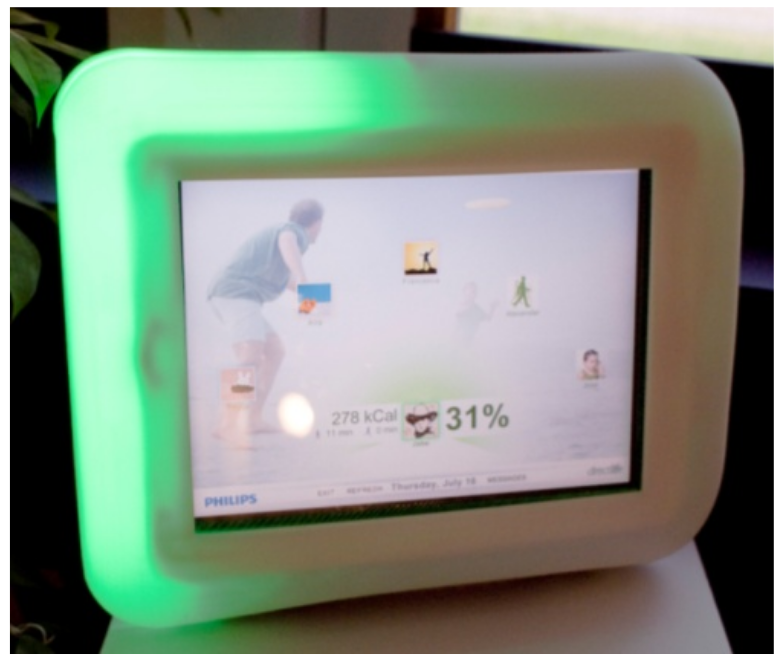
\includegraphics[width=0.900\hsize]{images/Aulura-screenshot2.png}
\caption{la zone \emph{Details} de \emph{Aulura}.}\label{fig:aulura2}
\end{figure*}

\paragraph{Étude}\label{uxe9tude-3}

Afin d'évaluer l'utilisabilité, l'esthétique et l'interactivité de
\emph{Aulura}, une étude a été effectuée dans un laboratoire simulant
l'environnement d'un foyer avec 16 participants (9 hommes, 7 femmes).
Les participants reçurent un détecteur d'activité physique capable de
communiquer avec \emph{Aulura} qu'ils devaient porter toute la journée
du test. Les participants durent choisir une couleur pour les identifier
et fournir 5 images personnelles qui furent ensuite affichées par
\emph{Aulura} pendant les tests. Les tests ont durées 90 minutes et les
participants ont participé à deux conditions : une avec l'affichage
ambiant et l'autre sans. Dans chaque condition les participants ont du
effectuer des tâches domestiques (e.g., faire une tasse de café ou lire
les pages d'un magazine) pour que l'interaction avec \emph{Aulura} soit
secondaire (voir Figure~\ref{fig:aulura2}).

\begin{figure*}
\centering
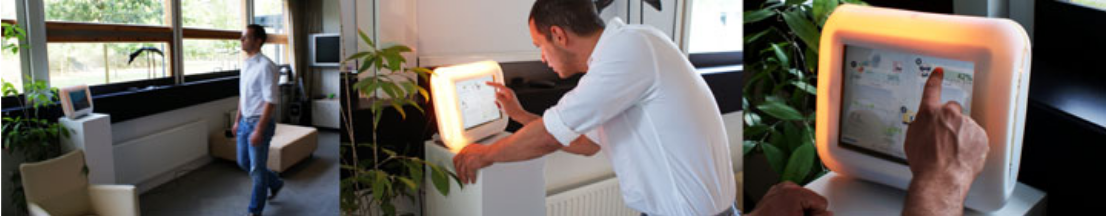
\includegraphics[width=0.900\hsize]{images/Aulura-screenshot1.png}
\caption{Un utilisateur interagit avec \emph{Aulura} pendant le test en
laboratoire}\label{fig:aulura2}
\end{figure*}

\paragraph{Recueil des données}\label{recueil-des-donnuxe9es-2}

À chaque fin de session, des données qualitatives furent collectées par
le biais d'une interview sur les différences d'utilisabilité,
d'esthétique et de persuasion entre les 2 conditions en relation avec .
Les questions incluaient est-ce que les utilisateurs ont remarqués et
compris les informations ambiantes ; est-ce que les différentes zones
d'interaction ont séduits les utilisateurs à se rapprocher du cadre et à
explorer plus d'informations ; et est-ce les utilisateurs partageraient
leurs informations personnelles avec leur famille et amis.

\paragraph{Analyse des données}\label{analyse-des-donnuxe9es-1}

Les interviews furent analysées par un diagramme d'affinité.

\paragraph{Résultats de l'analyse}\label{ruxe9sultats-de-lanalyse-1}

Les résultats clés donnent une première impression sur comment les
utilisateurs ont expérimentés le modèle d'interaction et l'esthétique
d'\emph{Aulura}. Pratiquement tout les participants (13 sur 16
personnes) ont remarqué et compris les informations ambiantes. Par
rapport à la condition sans l'affichage ambiant, les participants sont
plus motivés à vérifier leurs progrès.

\begin{itemize}
\item
  Santé et exercices
\item
  Économie, commerce, marketing, sécurité, sûreté -
  \citet{kalnikaite2011nudge} -.
\item
  Éducation, apprentissage - \citet{reis2011perception} -.
\item
  Gestion de l'énergie - \citet{belley2006semaphore},
  \citet{belley2006coupe}, \citet{evans2009artful},
  \citet{gustafsson2005power}, \citet{kyoto2005wattson},
  \citet{jonsson2010watt}, \citet{ernevi2005energy},
  \citet{gyllensward2006visualizing}, \citet{lagerkvist2016flower},
  \citet{lagerkvist2016disappearing}, \textcolor{red}{à lire}
  \citet{rogers2010ambient}, \citet{kuznetsov2010upstream},
  \citet{valkanova2013reveal} -.
\end{itemize}

\newpage
\bibliographystyle{apalike-fr}
\bibliography{resources/biblio}

\end{document}

